TODO intro


\subsection{CPUID Instruction}
\label{sec:approach-cpuid}

\mvf{Draft:}

P{\'e}k {\em et al.}~\cite{nether}

Ether alters the output of {\tt CPUID}, flipping the bit for TSC support. Should
be 1 in both VMM and bare metal environment. Can easily be checked, as shown in
Figure~\ref{fig:cpuid-tsc}, in the Appendix.

If it is a bug in the Ether implementation, best solution is to fix, though we
do not have good enough knowledge of the source code to know.

Alternatively, spoof the value in the same manner as {\tt PUSHF} and {\tt POPF}.
Ether deliberately changes the flag register when running, as it sets the debug
flag to be able to step through the target program and get a program trace. It
hides this from the target by spoofing the values of instructions used to read
and write these flags, as {\tt PUSHF} and {\tt POPF}. Figure~\ref{fig:pushf}
shows how the Xen hypervisor is patched to check for specific instructions and
alter the effect of that instruction. The exact same technique could be used to
spoof the TSC-bit when program executes CPUID.

This technique of spoofing the CPUID output suffers from timing attacks, which
will be elaborated in~\nameref{sec:approach-timing}.

\begin{figure}
\begin{lstc}
void vmx_set_pending_exceptions(struct vcpu *v)
{
    ...
+    if(instruction[0] == 0x9C)
+    {
+         /* detected PUSHF */
+
+         v->domain->arch.hvm_domain.ether_controls.send_guest_exception = 1;
+         v->domain->arch.hvm_domain.ether_controls.next_expected_rip = guest_rip + 1;
+    }
+    else if (instruction[0] == 0x9D)
+    {
+         /* detected POPF */
+         ...
+    }
    ...
}
\end{lstc}
\caption{\label{fig:pushf} Part of the patch Ether does on the }
\end{figure}

\subsection{CPU Errata}
\label{sec:approach-errata}
CPU errata refer to the collection of design defects or errors that may induce the CPU to behave differently from the published specification. Such CPU errata is strongly bound to CPU models and nEther exploits bugs in the Core 2 Duo family, called AH4 Erratum. The AH4 Erratum states that "\texttt{VERW/VERR/LSL/LAR} instructions may unexpectedly update the Last Exception Record(LER) MSR" and there is no planned fix for it. Concretely, \texttt{VERW} and \texttt{VERR} instructions verify whether the code or data segment specified with the source operand is readable (\texttt{VERR}) or writable (\texttt{VERW}) from the current privilege level. The \texttt{LAR} instruction loads access rights from a segment descriptor into a general purpose register, and the \texttt{LSL} instruction loads the unscrambled segment limit from the segment descriptor into a general-purpose register~\cite{intelsys}. This erratum is a design fault so its existence is unintended. Therefore, hardware-assisted-virtualization solutions (e.g., Xen) will not implement this erratum in the virtual CPUs of guests, because there is no need to mimic even unexpected system bugs. As a result, malware can detect hardware-assisted virtualization environment by executing those buggy instructions and checking whether LER MSR is unexpectedly updated or not. In other words, this attack cannot recognize the presence of Ether, but can reveal the hardware-virtualized runtime environment. \\

To thwart this attack completely, we should patch those buggy instructions or use another CPU, but It seems like infeasible and make no sense. So, we propose two practical method to mitigate this attack.

\begin{figure}[!h]
	\centering
	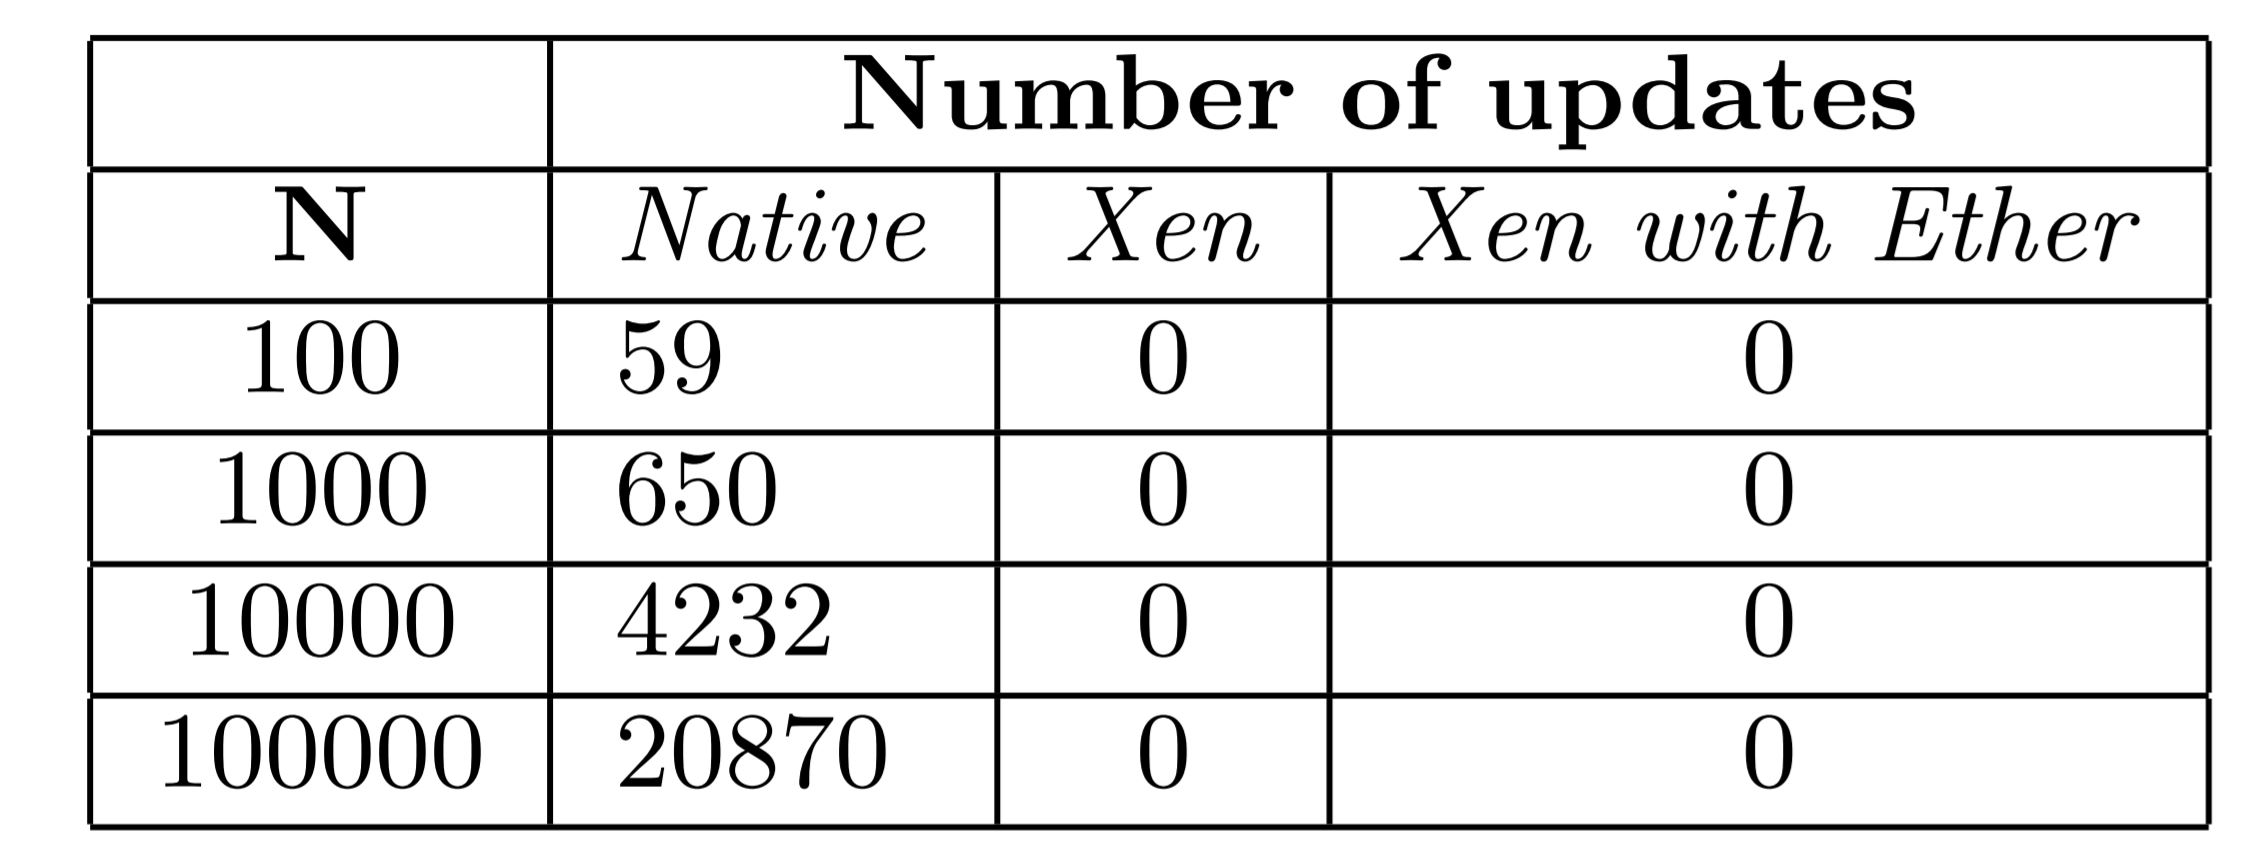
\includegraphics[width=\linewidth]{figure/errata_table.png}
	\caption{The number of LER MSR updates according to the erratum execution}
	\label{fig:errata}
\end{figure}

\subsubsection{Proposed Mitigation 1}
In general, those bugs do not happen always. Table~\ref{fig:errata} demonstrates the number of LER MSR updates when the CPU erratum was executed 100, 1000, 10000 and 100000 times under the corresponding environments. The update occurs only in the native environment, but the frequency of occurrence is unpredictable and irregular(from 20\% up to 65\%). Therefore, this CPU erratum should be executed in several times in order to detect hardware-assisted virtualization environment and this can be considered as a malicious behavior. So, to mitigate this attack, we set the threshold first and then count the number of all execution about those buggy instructions during the runtime of each program. If the counted number exceed the threshold, we can classify that program as a malware or just block to execute buggy instructions anymore. This method cannot prevent from CPU errata attack but can mitigate it, and there is a trade-off between TP and FP depending on how the threshold is set. Note that only kernel mode operations can access to LER MSR, therefore user mode operations does not need to be blocked or classified as a malware, even if execute the CPU erratum unlimited.

\subsubsection{Proposed Mitigation 2}
Another proposed mitigation is to mimic the CPU erratum intentionally. Our goal is to make it difficult to distinguish hardware-virtualized-environment from native one, and the attack exploits that LER MSR update happens only in native environment. Therefore, we may mitigate this attack by updating LER MSR intentionally whenever buggy instructions(\texttt{VERW/VERR/LSL/LAR}) are executed. This method can be implemented in two ways. The first one is to update LER MSR directly right after buggy instructions are executed while monitoring every kernel mode instructions. Note that we do not need to monitor user mode instructions, since attack code should be executed in kernel mode in order to read LER MSR and check whether it is updated or not. The second one is to add LER MSR update code right after every buggy instructions using binary rewriting. LER MSR is divided into {\tt MSR\_LER\_FROM\_LIP} and {\tt MSR\_LER\_TO\_LIP}, and those are located in {\tt 0x1dd} and {\tt 0x1de}, respectively. Therefore, we can add code to modify the value of {\tt0x1dd} and {\tt 0x1de} immediately after \texttt{VERW/VERR/LSL/LAR} instructions, as shown in the Figure~\ref{fig:wrmsr}. Such binary rewriting may be conducted only when kernel module is loaded in the memory in order to minimize performance overhead. This mitigation cannot be applied to self-modifying code, but it is out of scope in our paper.

\begin{figure}[h]
\begin{lstc}
__asm__ {
	/* wrmsr : MSR[ECX] = EDX:EAX; */
	...
	verr ax
+	/* store arbitary value in eax, edx */
+	mov ecx, 0x1dd
+	wrmsr 
+	mov ecx, 0x1de
+	wrmsr
	...
	verw cx
+	/* store arbitary value in eax, edx */
+	mov ecx, 0x1dd
+	wrmsr
+	mov ecx, 0x1de
+	wrmsr
	...
}

\end{lstc}
\caption{\label{fig:wrmsr} Code snippet in assembly showing how to rewrite binary for updating LER MSR intendedly. }
\end{figure}

\subsection{Timing Information}
\label{sec:approach-timing}
Taking advantage of the performance measures and timing information is more sophisticated method for malwares to detect its environment. Although virtual machine\textquotesingle s performance will always slower than it would have been on real hardware, blindly measuring the absolute performance scores is not sufficient to detect virtual environments.\cite{raffetseder2007} Generally, two approaches to use timing information.

\begin{figure*}[!t]
	\centering
	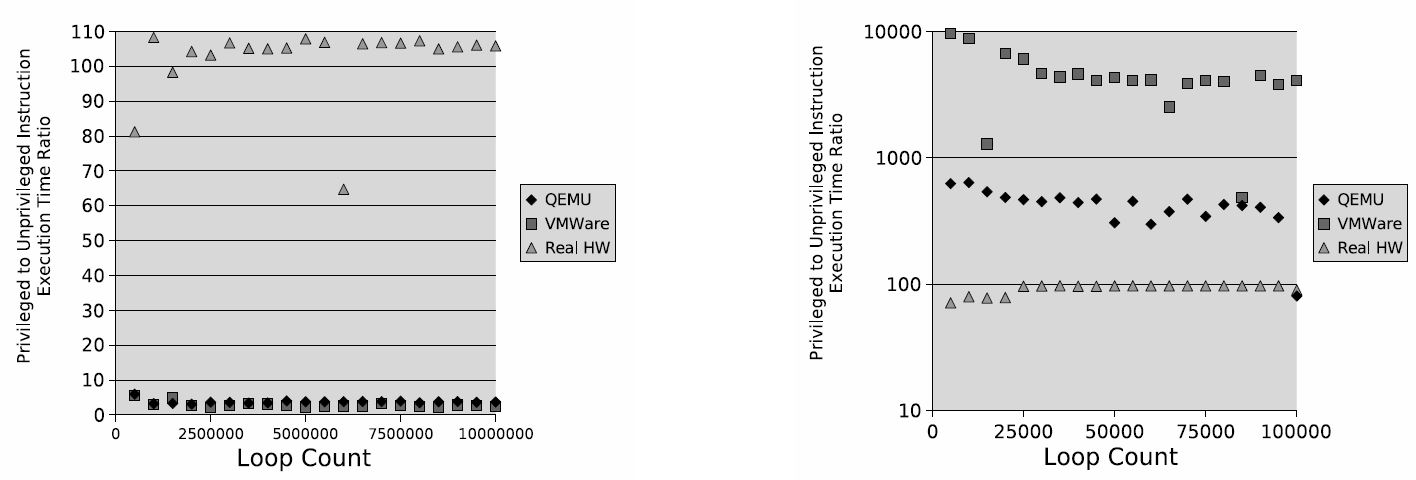
\includegraphics[width=\textwidth]{figure/comp_inst.jpg}
	\caption{Reading/Writing on CR0 (left) and CR3 (right)}
	\label{fig:comparison_of_instructions}
\end{figure*}

\subsubsection{Comparison of Instructions}
Even though a single performance score does not provide any meaningful clues, comparing the time taken between privileged instructions and unprivileged instructions can be useful to the VM detection mechanism. Raffetseder {\em et al.}~\cite{raffetseder2007} has used unprivileged instruction \textquotesingle s performance as a baseline and compare it privileged instruction \textquotesingle s to obtain relative performance number.
\begin{equation*}
Relative Performance = \frac{T_{privileged}}{T_{unprivileged}}
\end{equation*}
The insight is that real processors has to perform different tasks than simulated processors when handling privileged instructions. Thus it causes different relative performance results.  Raffetseder{\em et al.}~\cite{raffetseder2007} has conducted an experiment to prove the concept. A kernel module reads from a control register (CR0\footnote{contains various control flags} or CR3\footnote{When virtual addressing is enabled, CR3 register helps on virtual address to physical address translation}), then writes it back to where it came from. Raffetseder used processor\textquotesingle s time stamp counter (TSC) to measure the time elapsed to execute instructions. Figure~\ref{fig:comparison_of_instructions} shows the results. Real hardware showed poor relative performances when accessing CR0 but showed greater performance on CR3. Although Raffetseder did not explicitly explained why the results are different, it experiments showed a about difference in terms of 10 to 100 times between emulated and real environments. Thus, the difference is large enough to detect virtual environments.

\subsubsection{Mitigation of Comparison of Instructions}
Raffetseder\textquotesingle s~\cite{raffetseder2007} experiments on comparison of instructions were done on software based emulation solutions (e.g. Qemu, VMware, etc.) which are fundamentally more limited than hardware solutions (e.g. Intel VT-x). Intel VT-x that runs on Xen hypervisor provides \texttt{TSC\_OFFSET} (Timestamp-Counter Scaling Offset) field additional to the regular  \texttt{TSC} field that is specifically design to skew the guest time upon clock cycle requests. When the guest guest queries for the \texttt{TSC} value, the hypervisor would return the difference between the \texttt{TSC} and \texttt{TSC\_OFFSET} as the clock cycle. Since the \texttt{TSC\_OFFSET} is under control of the hypervisor, sandboxing the malware on hardware based virtual environment should mitigate the relative performance difference vulnerability.

\subsubsection{Cached Instructions}
Caching lets the system hold on to recently executed functions in case they are needed again in near future. As a result, executing cached functions will consume less CPU cycles compared to the first time as shown on Figure~\ref{fig:cache_realhw} left. However, caching can be turned off on machines running on bare metal by making the processor enter the no-fill cache mode and flushing out all existing caches by using the WBINVD instruction. As a result, latter executions consume as much CPU cycles as the first run as shown on Figure~\ref{fig:cache_realhw} right.
However, it was shown that disabling caching is not properly supported on Qemu and VMware. Raffetseder{\em et al.}~\cite{raffetseder2007} has executed six independent test runs where each test run consists of five calls to one function. Both the Qemu (Figure~\ref{fig:cache_qemu}) and VMware (Figure~\ref{fig:cache_vmware}) had significant CPU cycle reduction after the first execution regardless of the caching preference.
Therefore, malware authors can take advantage of the fact the caching cannot be turned off on virtual environments. If a malware obtain measurements similar to Figure~\ref{fig:cache_qemu} or Figure~\ref{fig:cache_vmware}, it should consider itself being in a sandbox and hide its malicious executions.


\begin{figure*}[!t]
	\centering
	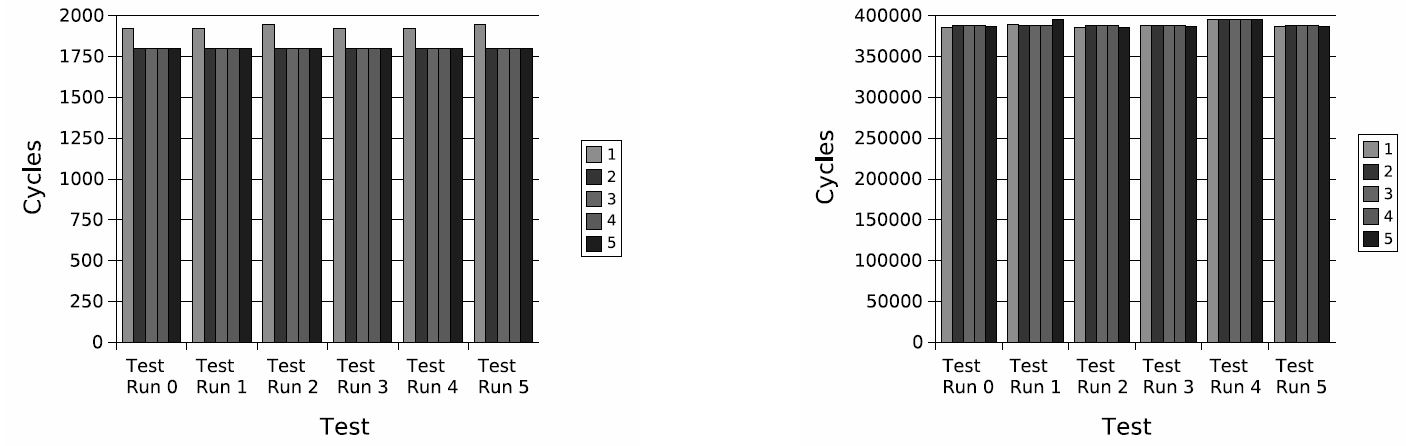
\includegraphics[width=\textwidth]{figure/realhw.jpg}
	\caption{Real hardware Cache On (left), Cache Off (right)}
	\label{fig:cache_realhw}
\end{figure*}

\begin{figure*}[!t]
	\centering
	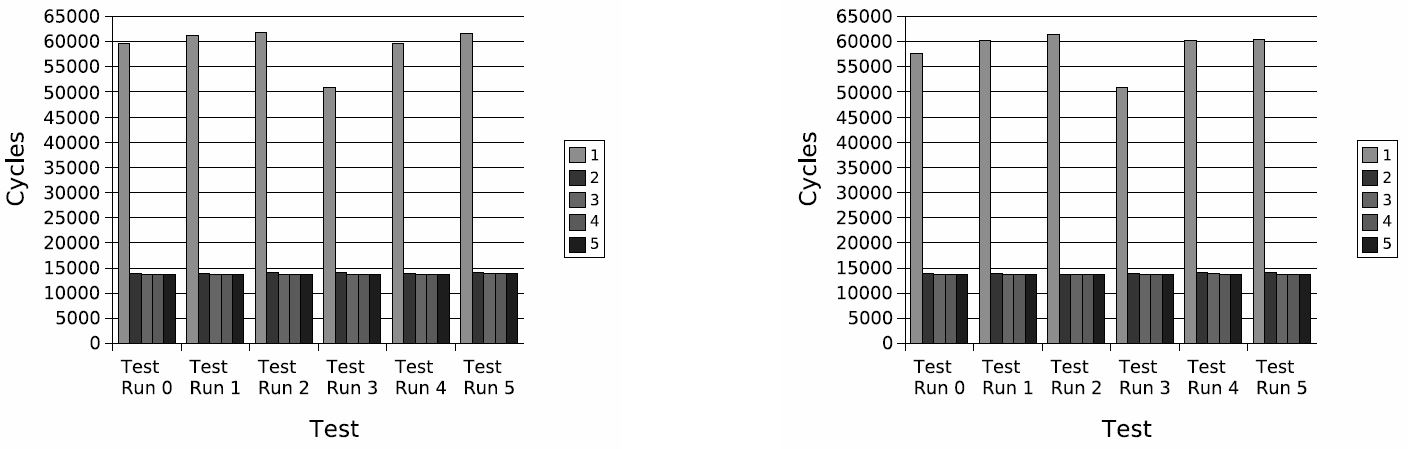
\includegraphics[width=\textwidth]{figure/qemu.jpg}
	\caption{Qemu On (left), Cache Off (right)}
	\label{fig:cache_qemu}
\end{figure*}

\begin{figure*}[!t]
	\centering
	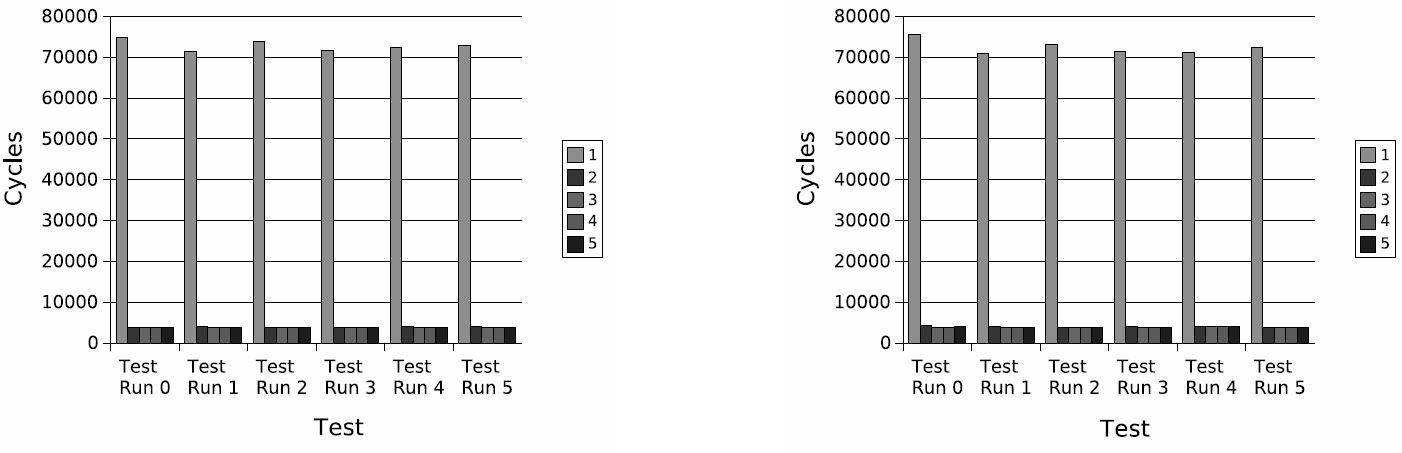
\includegraphics[width=\textwidth]{figure/vmware.jpg}
	\caption{VMware Cache On (left), Cache Off (right)}
	\label{fig:cache_vmware}
\end{figure*}

%%% Local Variables:
%%% mode: latex
%%% TeX-master: "../paper"
%%% End:
